\section{块编码的压缩极限}
\label{sec:lossless-block-limits}

逐符号编码的冗余可以接近一位，原因是每个符号至少花一位。把$n$个符号合成一块编码，可以从两个方向利用这一点。一是仍要求每块精确还原，但让整数码长的取整损失摊到$n$个符号上；二是放弃对极少数块的还原，只给高概率的块编号，从而使用固定长度的码字。两条路都把每符号所需的位数压到熵$H(X)$，但允许的码长形式和错误要求不同。本节设$X_1,X_2,\dots$独立同分布，服从字母表$\mathcal{X}$上的$p$。

\subsection{零错误的变长块编码}
\label{sec:lossless-variable-block}

把块$x_{1:n}$看作字母表$\mathcal{X}^n$中的一个符号，它的概率由式~\eqref{eq:lossless-product}给出。对这个大字母表直接应用定理~\ref{thm:lossless-entropy-bound}，需要知道块的熵。

\begin{lemma}[独立块的熵]
\label{lem:lossless-block-entropy}
若$X_1,\dots,X_n$独立同分布，则
\begin{equation}
 H(X_{1:n})=nH(X_1).
 \label{eq:lossless-block-entropy}
\end{equation}
\end{lemma}

\begin{proof}
由式~\eqref{eq:lossless-product}，块的自信息是各符号自信息之和：
\[
 -\log_2p(x_{1:n})=\sum_{i=1}^{n}\bigl(-\log_2p(x_i)\bigr).
\]
在$x_{1:n}$处取值为$X_{1:n}$，两边取期望，由期望的线性性与同分布，
\[
 \begin{aligned}
 H(X_{1:n})&=\mathbb{E}\Bigl[\sum_{i=1}^{n}-\log_2p(X_i)\Bigr]\\
 &=\sum_{i=1}^{n}H(X_i)=nH(X_1). \qedhere
 \end{aligned}
\]
\end{proof}

\begin{theorem}[变长块编码]
\label{thm:lossless-variable-block}
设$\lvert\mathcal{X}\rvert\geq2$，各$p(x)>0$，块长$n\geq1$。$\mathcal{X}^n$上平均码长最短的唯一可译码$c_n^{\star}$满足
\begin{equation}
 H(X)\leq\frac{L(c_n^{\star})}{n}<H(X)+\frac1n .
 \label{eq:lossless-block-bound}
\end{equation}
\end{theorem}

\begin{proof}
$\mathcal{X}^n$至少有两个元素，每个块的概率都是正的。对字母表$\mathcal{X}^n$与块的分布应用定理~\ref{thm:lossless-entropy-bound}，任何唯一可译码的平均码长不小于$H(X_{1:n})$，而按块的自信息取整的Shannon码平均码长小于$H(X_{1:n})+1$。最优码介于两者之间：
\[
 H(X_{1:n})\leq L(c_n^{\star})<H(X_{1:n})+1 .
\]
由式~\eqref{eq:lossless-block-entropy}代入$H(X_{1:n})=nH(X)$，再除以$n$即得。
\end{proof}

最优码$c_n^{\star}$可以用Huffman编码对$\lvert\mathcal{X}\rvert^n$个块求出。整数码长带来的不到一位的冗余是每块一次，摊到每个符号上不足$1/n$位。对确定源，第~\ref{sec:lossless-average-length}节的讨论照样适用：长度已知时什么都不必发送；长度未约定时，空码字无法区分块数。

\paragraph{贯穿例}
对贯穿例的$n=1,\dots,6$分别构造块上的Huffman码，每符号平均码长为
\[
 \begin{gathered}
 1.900,\quad 1.865,\quad 1.859,\\
 1.853,\quad 1.853,\quad 1.851 ,
 \end{gathered}
\]
都在$[1.846,\,1.846+1/n)$中。图~\ref{fig:lossless-block-huffman}(a)把它们与块上Shannon码的每符号平均码长一起画出。数列不一定单调：$n=5$的值$1.85347$略大于$n=4$的值$1.85323$。定理只保证上界$H+1/n$单调下降，最优冗余本身随块长的变化取决于块概率怎样与$2$的整数次幂对齐。

\begin{BookInlineFigure}
 \centering
 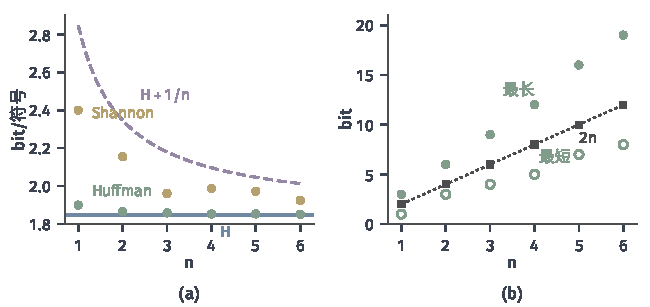
\includegraphics[width=110mm]{figures/07-probability/05-source-coding/matplotlib/lossless-block-huffman/figure.pdf}
 \caption{贯穿例的变长块编码，块长$n=1,\dots,6$。(a)每符号平均码长：绿点为块上的Huffman码，黄点为块上的Shannon码，蓝线为熵$H=1.846$，紫色虚线为上界$H+1/n$。(b)块上Huffman码的最短码字（空心绿点）与最长码字（实心绿点），灰色方点为同一块长的定长码$2n$位。}
 \label{fig:lossless-block-huffman}
\end{BookInlineFigure}

块编码对概率很不均匀的信源收益更大。第~\ref{sec:lossless-average-length}节的二元信源$\theta=0.1$，熵为$0.469$，逐符号编码至少要$1$位。块上Huffman码的每符号平均码长在$n=1,\dots,6$时为
\[
 \begin{gathered}
 1.000,\quad 0.645,\quad 0.533,\\
 0.493,\quad 0.480,\quad 0.470 ,
 \end{gathered}
\]
$n=6$时已与熵只差$0.001$位；$n=7$时反而回升到$0.474$。逐符号编码一半以上的位数是取整造成的，合成块以后这部分几乎全部收回。

\paragraph{平均保证不管最坏情形}
式~\eqref{eq:lossless-block-bound}是关于平均的。图~\ref{fig:lossless-block-huffman}(b)显示，块上Huffman码的最长码字随$n$增长得比定长码快：$n=6$时最长码字$19$位，而定长码只需$12$位；最长码字属于$dddddd$这样概率为$10^{-6}$的块。零错误的要求意味着这些罕见的块也必须有码字，它们只能放在码树的深处。

块编码的另外两项代价不在式~\eqref{eq:lossless-block-bound}中。一是码本：块上的码表有$4^n$项，$n=6$时为$4096$项，编码器与解码器都要存储，若码表要随消息一起传送，还要计入它的描述长度。二是构造与查找：Huffman构造需要$O(4^n\cdot n)$次比较。所以“块越长越接近熵”只在不计码本与计算代价时成立，第~\ref{sec:lossless-finite-resources}节把这些代价放在一起比较。

\subsection{允许错误的定长块编码}
\label{sec:lossless-fixed-block}

现在换一种要求：码字都等长，每块用同样多的位，但允许极少数块无法还原。这时问题变成“需要给多少个块编号”。四符号信源长度为$n$的块共有$4^n$个，全部编号需要$2n$位；如果绝大部分概率集中在少得多的块上，只给这些块编号就够了。

\begin{definition}[定长块编码与码率]
\label{def:lossless-fixed-length}
块长为$n$、含$M_n$个码字的定长块编码由编码映射$f_n:\mathcal{X}^n\to\{1,\dots,M_n\}$与解码映射$g_n:\{1,\dots,M_n\}\to\mathcal{X}^n$组成。每个编号用$\lceil\log_2M_n\rceil$位表示，\term{码率}（code rate）定义为
\begin{equation}
 R_n=\frac{\log_2M_n}{n}
 \label{eq:lossless-rate}
\end{equation}
单位是bit每源符号。错误概率为
\begin{equation}
 P_{\mathrm{e}}^{(n)}=\mathbb{P}\bigl(g_n(f_n(X_{1:n}))\neq X_{1:n}\bigr).
 \label{eq:lossless-error-prob}
\end{equation}
\end{definition}

\paragraph{自信息的集中}
要找出“概率集中在哪些块上”，先看一个块的每符号自信息$-\frac1n\log_2p(X_{1:n})$。由引理~\ref{lem:lossless-block-entropy}的证明，它是$n$个独立同分布随机变量
\[
 Y_i=-\log_2p(X_i)
\]
的样本平均。$Y_i$只取有限个值，均值是$H(X)$，方差
\[
 \sigma^2=\operatorname{Var}(Y_1)=\sum_xp(x)\bigl(-\log_2p(x)-H(X)\bigr)^2
\]
有限。第~\ref{chap:laws-of-large-numbers}章的弱大数律于是给出下面的结论。

\begin{theorem}[渐近均分性]
\label{thm:lossless-aep}
设$X_1,X_2,\dots$独立同分布，取值于有限字母表，各$p(x)>0$。则对每个$\varepsilon>0$，
\begin{equation}
 \mathbb{P}\Bigl(\Bigl\lvert-\frac1n\log_2p(X_{1:n})-H(X)\Bigr\rvert\geq\varepsilon\Bigr)\leq\frac{\sigma^2}{n\varepsilon^2}\xrightarrow[n\to\infty]{}0 .
 \label{eq:lossless-aep}
\end{equation}
\end{theorem}

\begin{proof}
$-\frac1n\log_2p(X_{1:n})=\frac1n\sum_iY_i$，其期望为$H(X)$，方差为$\sigma^2/n$。对它用第~\ref{chap:tail-probabilities}章的Chebyshev不等式即得。
\end{proof}

这一性质称为\term{渐近均分性}（asymptotic equipartition property）。名称的含义是：$n$大时，实际出现的块几乎都满足
\[
 p(x_{1:n})\approx2^{-nH(X)},
\]
即它们的概率“近似相等”，都在$2^{-n(H\pm\varepsilon)}$之间。这并不是说最可能的块概率接近$2^{-nH}$：贯穿例中最可能的块$aa\cdots a$的概率是$0.4^n=2^{-1.32n}$，远大于$2^{-1.85n}$；只是这样的块太少，合起来的概率可以忽略。

图~\ref{fig:lossless-aep-concentration}画出贯穿例中每符号自信息的精确分布。它按块中$a,b,c,d$的个数枚举所有类型，逐类求和得到，没有用到模拟。$n=10$时分布还很宽，落在$H\pm0.1$内的概率只有$0.337$；$n=250$时，这一概率升到$0.990$。

\begin{BookInlineFigure}
 \centering
 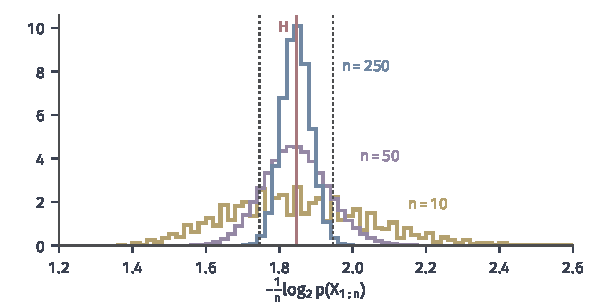
\includegraphics[width=100mm]{figures/07-probability/05-source-coding/matplotlib/lossless-aep-concentration/figure.pdf}
 \caption{贯穿例中每符号自信息$-\frac1n\log_2p(X_{1:n})$的精确分布，按宽$0.02$的格子汇总，纵轴为单位长度上的概率。黄、紫、蓝分别为$n=10,50,250$；红线为熵$H=1.846$，灰色虚线为$H\pm0.1$。}
 \label{fig:lossless-aep-concentration}
\end{BookInlineFigure}

\paragraph{典型集}
把每符号自信息接近熵的块收集起来。

\begin{definition}[典型集]
\label{def:lossless-typical-set}
对$\varepsilon>0$，称
\begin{equation}
 A_{\varepsilon}^{(n)}=\Bigl\{x_{1:n}\in\mathcal{X}^n:\ \Bigl\lvert-\frac1n\log_2p(x_{1:n})-H(X)\Bigr\rvert<\varepsilon\Bigr\}
 \label{eq:lossless-typical-set}
\end{equation}
为\term{典型集}（typical set）。
\end{definition}

等价地，$x_{1:n}\in A_{\varepsilon}^{(n)}$当且仅当
\[
 2^{-n(H(X)+\varepsilon)}<p(x_{1:n})<2^{-n(H(X)-\varepsilon)},
\]
即典型块的概率被夹在两个以熵为指数的数之间。

\begin{lemma}[典型集的性质]
\label{lem:lossless-typical-properties}
在定理~\ref{thm:lossless-aep}的条件下：
\begin{enumerate}
 \item 典型集的概率满足
 \begin{equation}
  \mathbb{P}\bigl(X_{1:n}\in A_{\varepsilon}^{(n)}\bigr)\geq1-\frac{\sigma^2}{n\varepsilon^2},
  \label{eq:lossless-typical-prob}
 \end{equation}
 从而趋于$1$；
 \item 典型集的大小满足
 \begin{equation}
  \lvert A_{\varepsilon}^{(n)}\rvert<2^{n(H(X)+\varepsilon)};
  \label{eq:lossless-typical-upper}
 \end{equation}
 \item 若典型集的概率不小于$1-\delta$，则
 \begin{equation}
  \lvert A_{\varepsilon}^{(n)}\rvert>(1-\delta)\,2^{n(H(X)-\varepsilon)}.
  \label{eq:lossless-typical-lower}
 \end{equation}
\end{enumerate}
\end{lemma}

\begin{proof}
第一条是式~\eqref{eq:lossless-aep}取补事件，即式~\eqref{eq:lossless-typical-prob}。第二条：典型集中每个块的概率都大于$2^{-n(H+\varepsilon)}$，它们的概率之和不超过$1$，所以
\[
 1\geq\sum_{x_{1:n}\in A_{\varepsilon}^{(n)}}p(x_{1:n})>\lvert A_{\varepsilon}^{(n)}\rvert\,2^{-n(H+\varepsilon)} .
\]
第三条：典型集中每个块的概率都小于$2^{-n(H-\varepsilon)}$，所以
\[
 1-\delta\leq\sum_{x_{1:n}\in A_{\varepsilon}^{(n)}}p(x_{1:n})<\lvert A_{\varepsilon}^{(n)}\rvert\,2^{-n(H-\varepsilon)} .
\]
整理即得。
\end{proof}

引理说明典型集“小而重”：它的元素个数大约是$2^{nH}$，只占全部$2^{n\log_2\lvert\mathcal{X}\rvert}$个块中的指数小部分，却几乎承载了全部概率。贯穿例中$\log_2 4=2$而$H=1.846$，比例约为
\[
 2^{-n(2-1.846)}=2^{-0.154n},
\]
$n=250$时约为$2^{-38}$。

式~\eqref{eq:lossless-typical-lower}说明上界~\eqref{eq:lossless-typical-upper}在指数上不能再改进：典型集至少要有约$2^{n(H-\varepsilon)}$个元素。图~\ref{fig:lossless-typical-set}给出$\varepsilon=0.1$时的精确数值。左图中典型集的概率随$n$上升，$n=230$时为$0.987$，远高于Chebyshev下界；右图中$\frac1n\log_2\lvert A_{\varepsilon}^{(n)}\rvert$落在$H\pm\varepsilon$之间，并明显低于$\log_24=2$。它靠近上端$H+\varepsilon$而不是$H$，是因为自信息较大的块数目多得多，典型集中的块大部分来自区间的上端。

\begin{BookInlineFigure}
 \centering
 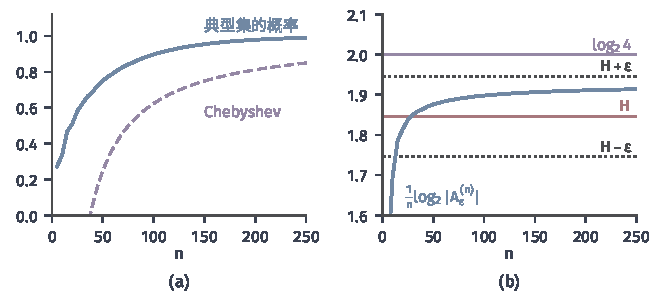
\includegraphics[width=110mm]{figures/07-probability/05-source-coding/matplotlib/lossless-typical-set/figure.pdf}
 \caption{贯穿例的典型集，$\varepsilon=0.1$，由类型枚举精确计算。(a)典型集的概率（蓝）与Chebyshev下界$1-\sigma^2/(n\varepsilon^2)$（紫色虚线），$\sigma^2=0.377$。(b)$\frac1n\log_2\lvert A_{\varepsilon}^{(n)}\rvert$（蓝），红线为$H$，灰色虚线为$H\pm\varepsilon$，紫线为全部块的$\log_24=2$。}
 \label{fig:lossless-typical-set}
\end{BookInlineFigure}

\paragraph{码率高于熵时可以做到}
典型集直接给出一种定长块编码：给典型集中的块逐个编号，另外留一个编号给所有非典型块。图~\ref{fig:lossless-typical-scheme}画出这一方案。

\begin{BookInlineFigure}
 \centering
 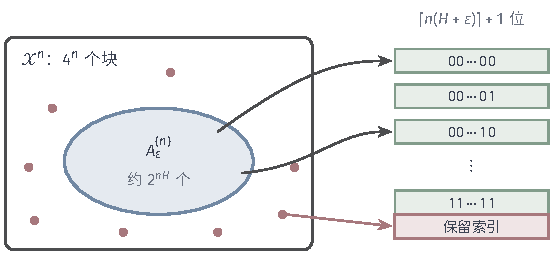
\includegraphics[width=94mm]{figures/07-probability/05-source-coding/tikz/lossless-typical-scheme/figure.pdf}
 \caption{用典型集构造定长块编码。左框为全部$4^n$个块，蓝色区域为典型集$A_{\varepsilon}^{(n)}$，约有$2^{nH}$个块；右侧绿格为等长的编号，每个典型块得到一个编号。红点为非典型块，全部送到红色的保留编号，解码时无法还原。}
 \label{fig:lossless-typical-scheme}
\end{BookInlineFigure}

\begin{theorem}[定长块编码的可达性]
\label{thm:lossless-fixed-achievability}
在定理~\ref{thm:lossless-aep}的条件下，对任意$R>H(X)$，存在一列定长块编码，其码率$R_n\leq R$（$n$充分大），错误概率$P_{\mathrm{e}}^{(n)}\to0$。
\end{theorem}

\begin{proof}
取$\varepsilon=(R-H(X))/2>0$。令编码映射把典型集中的块一一对应到编号$1,\dots,\lvert A_{\varepsilon}^{(n)}\rvert$，把其余块都映到编号$M_n=\lvert A_{\varepsilon}^{(n)}\rvert+1$；解码映射把前面的编号映回对应的典型块，把保留编号映到任意固定的块。由式~\eqref{eq:lossless-typical-upper}，
\[
 M_n<2^{n(H+\varepsilon)}+1\leq2^{n(H+2\varepsilon)}=2^{nR}
\]
在$n$充分大时成立，所以$R_n\leq R$。典型块都被正确还原，错误只可能发生在非典型块上，按式~\eqref{eq:lossless-error-prob}与式~\eqref{eq:lossless-typical-prob}，
\[
 P_{\mathrm{e}}^{(n)}\leq\mathbb{P}\bigl(X_{1:n}\notin A_{\varepsilon}^{(n)}\bigr)\leq\frac{\sigma^2}{n\varepsilon^2}\to0 . \qedhere
\]
\end{proof}

\paragraph{码率低于熵时做不到}
反过来，若码率低于熵，无论怎样选择要编号的块，错误概率都不能趋于零，实际上趋于$1$。

\begin{theorem}[定长块编码的逆定理]
\label{thm:lossless-fixed-converse}
在定理~\ref{thm:lossless-aep}的条件下，设$R<H(X)$，定长块编码满足$M_n\leq2^{nR}$。则$P_{\mathrm{e}}^{(n)}\to1$。
\end{theorem}

\begin{proof}
解码映射只有$M_n$个输出，能被正确还原的块组成集合
\[
 B_n=\{x_{1:n}:\ g_n(f_n(x_{1:n}))=x_{1:n}\},
\]
它的元素都在$g_n$的值域中，所以$\lvert B_n\rvert\leq M_n\leq2^{nR}$。取$\varepsilon=(H(X)-R)/2>0$，把正确还原的概率按是否典型拆开：
\[
 \mathbb{P}(X_{1:n}\in B_n)\leq\mathbb{P}\bigl(X_{1:n}\in B_n\cap A_{\varepsilon}^{(n)}\bigr)+\mathbb{P}\bigl(X_{1:n}\notin A_{\varepsilon}^{(n)}\bigr).
\]
第一项中每个块的概率小于$2^{-n(H-\varepsilon)}$，块的个数不超过$2^{nR}$，所以
\[
 \mathbb{P}\bigl(X_{1:n}\in B_n\cap A_{\varepsilon}^{(n)}\bigr)<2^{nR}\,2^{-n(H-\varepsilon)}=2^{-n\varepsilon}.
\]
第二项不超过$\sigma^2/(n\varepsilon^2)$。两项都趋于零，所以正确还原的概率趋于零，从而
\[
 P_{\mathrm{e}}^{(n)}=1-\mathbb{P}(X_{1:n}\in B_n)\to1. \qedhere
\]
\end{proof}

两个定理合起来说明，定长块编码能以趋于零的错误概率工作，当且仅当码率超过熵（$R=H$这一临界情形，上面的论证不作结论）。图~\ref{fig:lossless-fixed-rate-error}给出贯穿例中最好的定长码的错误概率：对给定的$M_n=\lfloor2^{nR}\rfloor$，编号给概率最大的$M_n$个块时错误概率最小。$R=1.95$时错误概率从$n=4$的$0.0157$降到$n=228$的$5.4\times10^{-5}$；$R=1.75$时，即使挑选最可能的块，错误概率仍从$0.160$升到$0.956$。

\begin{BookInlineFigure}
 \centering
 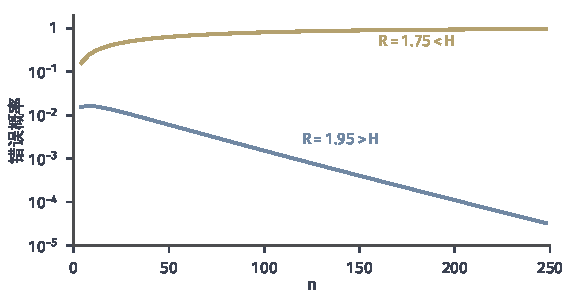
\includegraphics[width=96mm]{figures/07-probability/05-source-coding/matplotlib/lossless-fixed-rate-error/figure.pdf}
 \caption{贯穿例中码率为$R$的最优定长块编码的错误概率，纵轴为对数坐标。编码给概率最大的$\lfloor2^{nR}\rfloor$个块编号，其余块出错；数值由类型枚举精确计算。蓝线$R=1.95>H$，黄线$R=1.75<H$，$H=1.846$。}
 \label{fig:lossless-fixed-rate-error}
\end{BookInlineFigure}

\paragraph{错误来自哪里}
可达性定理中的错误全部来自非典型块，这些块合起来的概率很小。对单个块而言，结论是“要么精确还原，要么完全失败”：典型块精确还原，非典型块（例如$aa\cdots a$，以及$dd\cdots d$）一律出错。所以定理不能理解为“每条消息都能以接近熵的码率无损还原”。也不能理解为有限的$n$下错误概率已经可以忽略：贯穿例中$R=1.95$、$n=100$时错误概率仍有$1.5\times10^{-3}$。需要每条消息都还原时，应当用上一小节的变长块编码，它把这些罕见的块放到很长的码字里，而不是放弃它们。
